\section{Requirements}
All vtk files and rendered images can be found in the ./out folder. 
In order to build and run the project the following software packages are required
\begin{itemize}
    \item GCC compiler
    \item Python 3.8.5 or higher
    \item pyvista (for running display.py)
    \item pdflatex (to build the documentation)
\end{itemize}

While ParaView can be used to examine the vtk output files, pyvista is used to render images for the documentation by  invoking a python scriot (display.py)
PyVista still uses the vtk framework as a backend but offers a simple API for rendering files. This way the process of integrating simulation results into the documentation can be automated.

\section{Task 1 - Do you want to Build a Snowman?}
\subsection{Advercting a single sphere}
In this task the combination of multiple shapes and advections is explored.
We start by creating a single sphere and use a constant velociy field to shrink it.

\begin{minipage}{\linewidth}
\begin{lstlisting}[caption=Sphere creation and advection]
// create sphere
auto sphere1 = lsSmartPointer<lsDomain<NumericType, D>>::New(gridDelta);
{

    NumericType origin[3] = {0., 0., 0.};
    NumericType radius = 10.0;
    lsMakeGeometry<NumericType, D>(
        sphere1,
        lsSmartPointer<lsSphere<NumericType, D>>::New(
            origin, 
            radius)
        ).apply(); 
}

lsAdvect<double, D> advectionKernel;
auto constant_vf = lsSmartPointer<ConstantVelocityField>::New(-1);

advectionKernel.insertNextLevelSet(sphere1);
advectionKernel.setVelocityField(constant_vf);
advectionKernel.apply(); 

double advectionSteps = advectionKernel.getNumberOfTimeSteps();
std::cout << Number of Advection steps taken:  << advectionSteps << endl;

>> Number of Advection steps taken: 28
\end{lstlisting}
\end{minipage}

\begin{figure}[h]
    % Rigth image
    \begin{subfigure}{0.45\textwidth}
    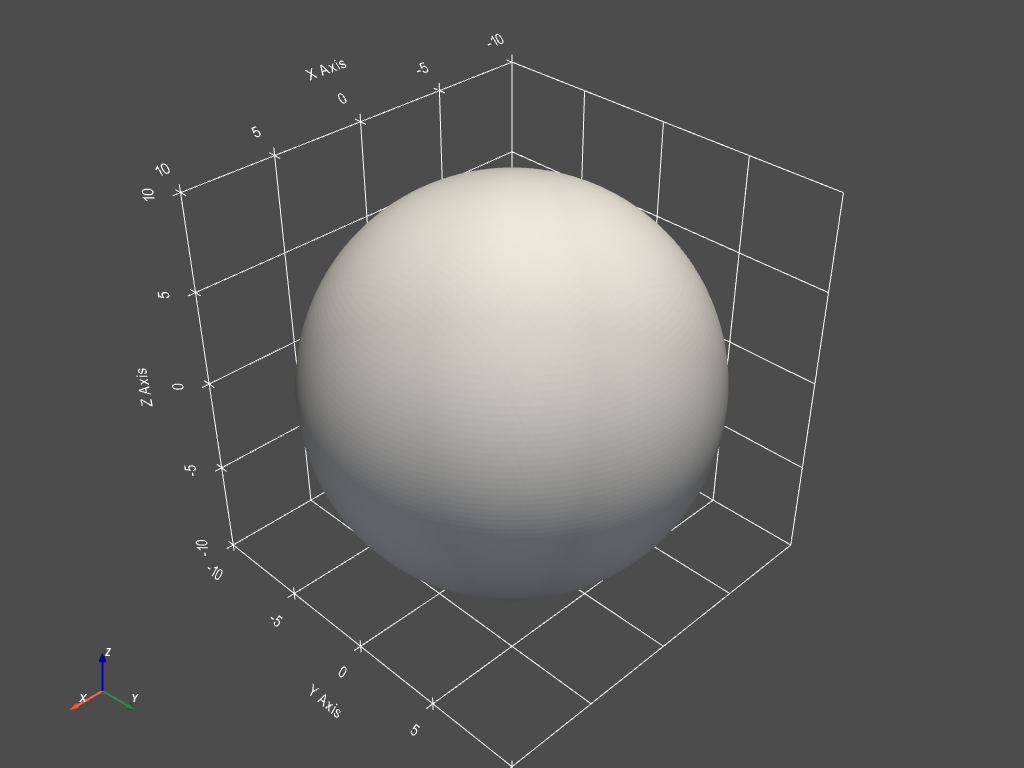
\includegraphics[width=1\linewidth]{res/task1.1_sphere1.png} 
    \caption{The initial sphere}
    %\label{fig:serial-solution}
    
\end{subfigure}
    % left image
    \begin{subfigure}{0.45\textwidth}
    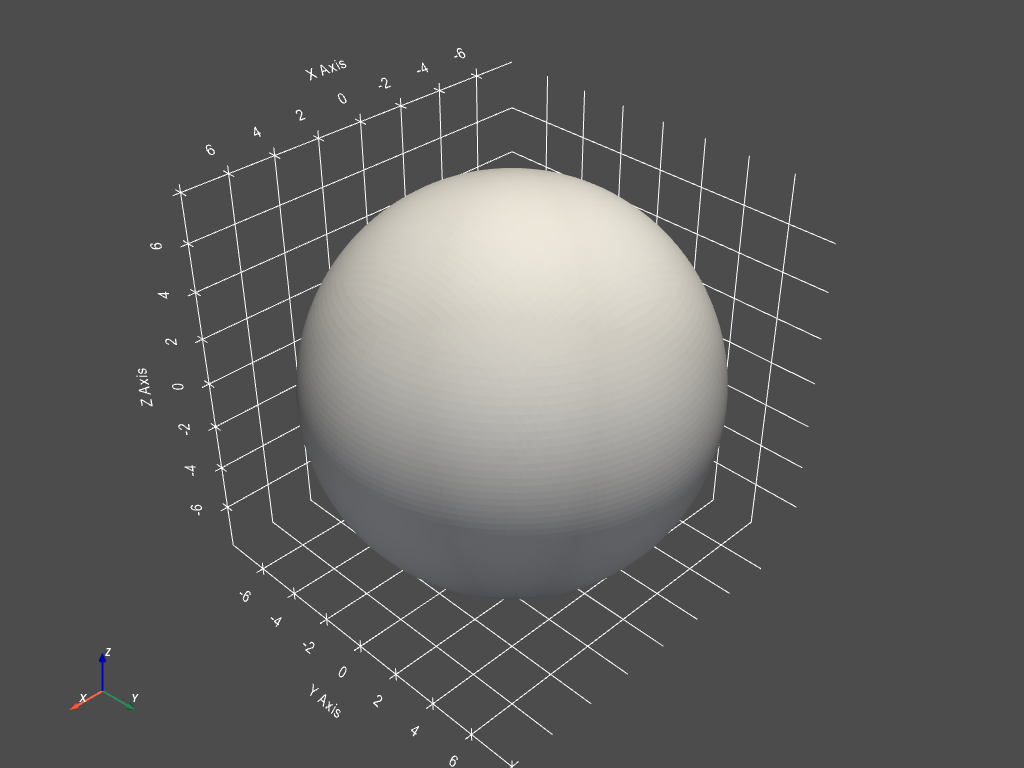
\includegraphics[width=1\linewidth]{res/task1.1_sphere2.png}
    \caption{The sphere after advection}
    %\label{fig:parallel-solution}
\end{subfigure}

\caption{Shrinking a sphere by constant advection. Note that both images use different grid spacings. A positive velocity would result in an expanding sphere (not depicted).}
\label{fig:task1.1_spheres}
\end{figure}

Fig. \ref{fig:task1.1_spheres} shows the sphere with an initial radius = 10 before and after advection. 
The difference in size can be read from the grid axes. A constant velocity field of -2 is used to shrink the object over the period of 1 unit of time. 
Therefore each point has to move 2 units of space towards the center, ths resulting in a new radius = 6.

The results coincide with the expectations and the advection seems to be stable.

\subsection{Combining multiple spheres}
Next multiple spheres are combined to construct a snowman. 
Then a constant velocty field is applied to simulate uniform melting/etching.

\begin{figure}[h]
    % Rigth image
    \begin{subfigure}{0.45\textwidth}
    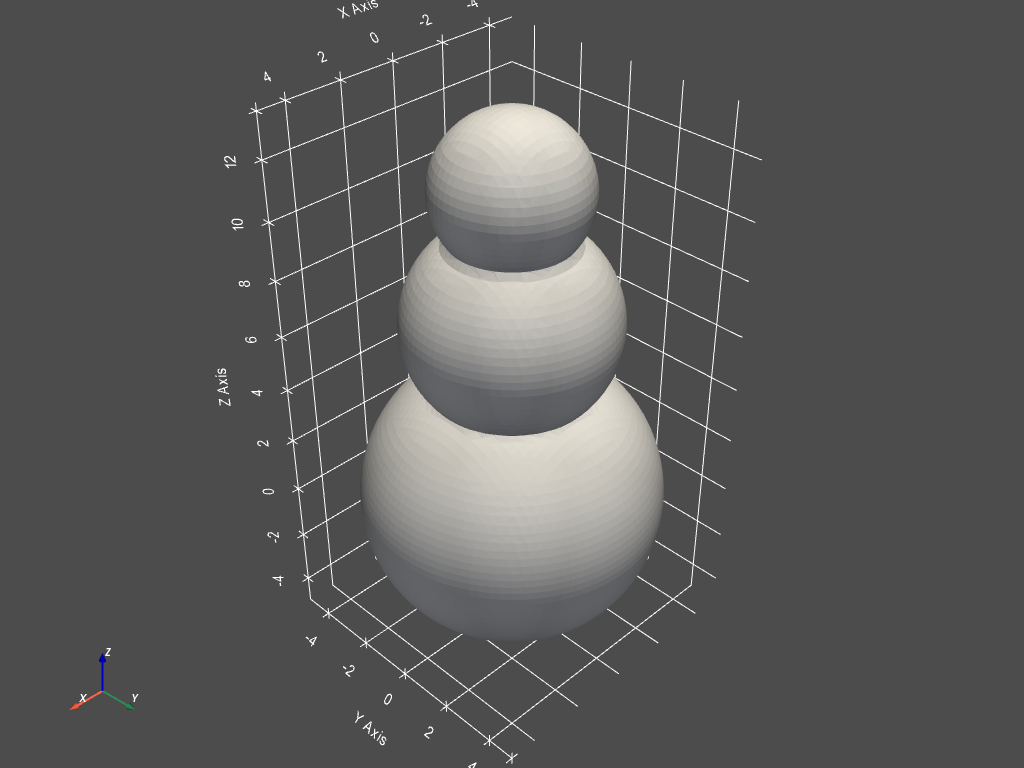
\includegraphics[width=1\linewidth]{res/task1.3_snowman1.png} 
    \caption{The initial snowman}
    
\end{subfigure}
    % left image
    \begin{subfigure}{0.45\textwidth}
    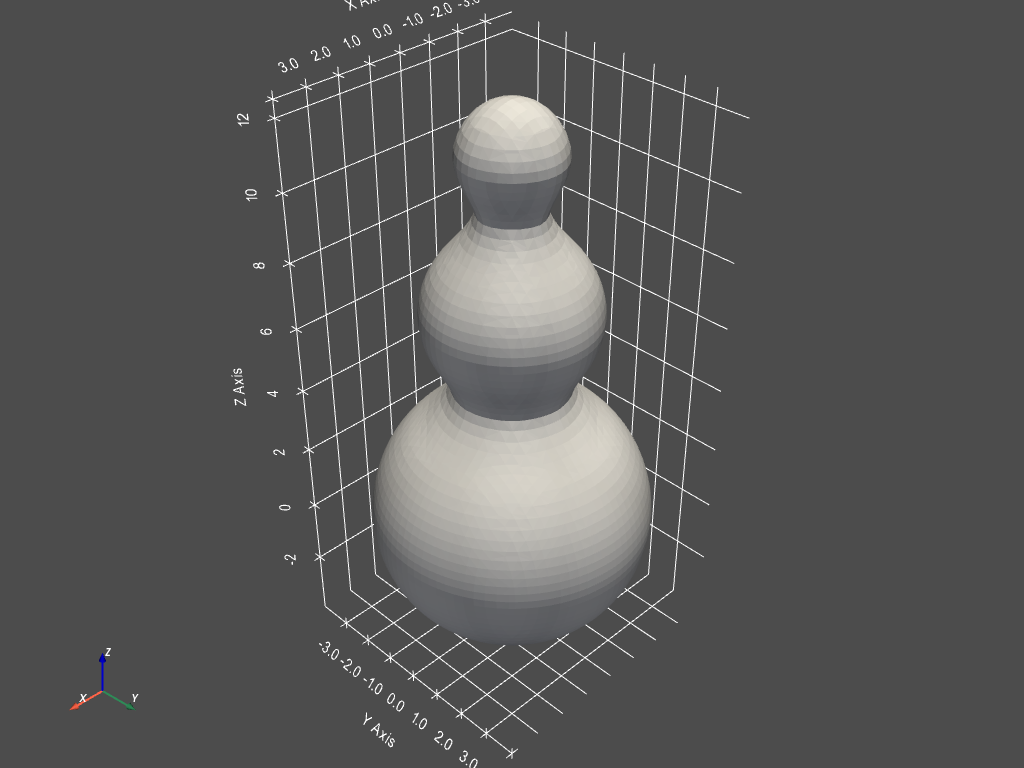
\includegraphics[width=1\linewidth]{res/task1.3_snowman2.png}
    \caption{The snowman after melting}
\end{subfigure}

\caption{Melting a snowman consisting of multiple spheres. Sharp edges where the initial spheres touch become rounded by the advection.}
\end{figure}